\section{The RationalGRL Methodology and Tool Support}
\label{sect:meth+tool}

In the previous sections, we have shown how the RationalGRL framework can capture stakeholder discussions, and how interactions between two types of reasoning, practical reasoning and goal modeling, leads to two interlinked models, RationalGRL and GRL models. In this section we clarify how practitioners can actually use the RationalGRL framework by proposing a methodology\footnote{The methodology presented here was first presented at the 2017 iStar workshop \cite{iSTar}.} (\textbf{requirement 4}) and discussing a prototype RationalGRL tool (\textbf{requirement 5}).

\subsection{RationalGRL Methodology}
\label{sect:methodology} 

We propose the methodology shown in Figure~\ref{fig:rationalgrl-methodology} to develop a (Rational)GRL model. %Here we assume that the initial GRL models have been created based on the requirements specification documents and the discussions of the stakeholders. The rest of the steps are as follows:

\begin{figure*}[ht]
\centering
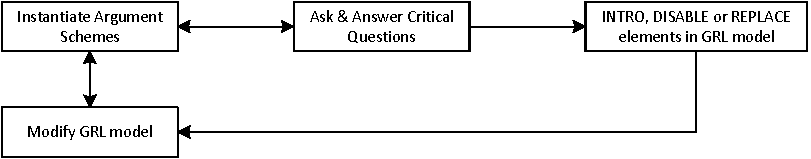
\includegraphics{img/methodology.pdf}
\caption{The RationalGRL Methodology}
\label{fig:rationalgrl-methodology}
\end{figure*}

\textbf{(1) Instantiate Argument Schemes (AS)} -- First, we start with our list of argument schemes (Table~\ref{table:argument-schemes}). Whilst discussing the requirements, we then select schemes from the list and instantiate them to form arguments for GRL model elements. In this way we build or modify the GRL model by introducing new GRL elements (\textsf{INTRO}, see example 1 in Section~\ref{sect:overview:examples}). Note that it is also possible to start modifying an existing GRL model which was not built using the RationalGRL methodology: each GRL element corresponds to an argument (i.e. an instantiated scheme), so it is possible to instantiate argument schemes based on an existing GRL model. 

\textbf{(2) Answer Critical Questions (CQs)} -- After building or modifying the initial GRL model, we can start asking the relevant critical questions. Because each element in the GRL model corresponds to an instantiated scheme, we can look at Table~\ref{table:argument-schemes}) to see which questions are relevant given our GRL model. 

\textbf{(3) Decide on Intentional Elements and their Relationships} -- By answering a critical question, one of three operations are performed on the GRL model: \textsf{INTRO}, \textsf{DISABLE} or \textsf{REPLACE}. Any of these operations impact the arguments and corresponding GRL intentional elements, modifying the initial GRL model into a RationalGRL model (see examples in Section~\ref{sect:overview:examples}). After these modifications, we can keep on asking critical questions (e.g. about elements that were introduced by previously answering a critical question) until we are satisfied with our model.   

\textbf{(4) Modify GRL Models} -- In this step, we modify the regular GRL model based on the RationalGRL model of step (3). That is, one of the following situation can happen with respect to the initial GRL model: 1) a new intentional element or a new link is introduced; 2) an existing intentional element or an existing link gets disabled (removed) from the model; or 3) an existing intentional element or link is replaced by a new one. This results in a new, modified GRL model, which can be used as the basis for another cycle of the methodology. 

We can continue these four steps until there is no more intentional element or link to analyze or we reach a satisfactory model. In the next section, we will give an example of how our tool can be used together with the methodology to build a GRL model.  

\iffalse%%%%%%%%%%%%%%%%%%%%%%%%%%%%%%%%%%%%%%%%%%%%%%%%%%%%%%%%%%%
\subsubsection{Example 6: Methodology example}

In this section, we present a small example for the RationalGRL methodology. This example is based on the traffic simulator example described in Section~\ref{sect:goals:runningexample}. We base argument schemes and critical questions of this example on a transcript containing discussions about the development of this traffic simulator system. %These transcripts are created as part of two master theses on improving design reasoning~\cite{masterthesis1,masterthesis2}. %TODO again?
%We provide several more examples in Section~\ref{sect:examples}.

As mentioned in Section~\ref{sect:goals:runningexample}, a group of stakeholders are developing a goal model for a traffic simulator example and they are modeling the goal \emph{Simulate Traffic} using the RationalGRL methodology. This proceeds in the following way:
\begin{itemize}
\item
First they start %at step \emph{Modify GRL models} (Figure~\ref{fig:rationalgrl-methodology}), 
with the initial GRL model (Figure~\ref{fig:example-small}) and they invoke the intentional element \emph{Simulate Traffic}. 
\item Next, they switch to the argumentation part (step \emph{Instantiate arguments schemes}). They answer critical question \emph{Does Simulate Traffic AND-decompose into any tasks?} with \emph{Yes: namely tasks ``Dynamic Simulation'' and ``Static Simulation"}.
\item As a result, two argument schemes are created, namely:
\begin{itemize}
\item Actor \emph{Traffic Simulator} has task \emph{Dynamic Simulation}
\item Actor \emph{Traffic Simulator} has task \emph{Static Simulation}
\end{itemize}
\item In the GRL model, this corresponds to the addition of two tasks, and an AND-decomposition from the goal \emph{Simulate Traffic} to these two tasks.
\item Next, the stakeholders test the validity of their goal model by answering more critical question. They answer two critical questions:
\begin{itemize}
\item
CQ \emph{Is task ``Dynamic Simulation'' relevant} is answered with ``No, it is not relevant since the problem specification explicitly states dynamic simulations are not required''. Thus, the corresponding GRL intentional element is disabled.
\item The decomposition is changed from AND to OR, since it turned out not both tasks can be implemented together.
\end{itemize}
\end{itemize}

An excerpt of the RationalGRL model is shown in Figure~\ref{fig:examples:decomposition}. %TODO You need to update goal "simulate" in this figure to "Simulate Traffic".  Also, I don't think we should really call it the rational GRL model. it is an excerpts of the model. 
\fi

\subsection{The RationalGRL Tool}
\label{sect:tool}
\todo{Marc}{Marc}{Currently this section comes from my thesis where I present the tool as future work. Here we should explain it}

GRL has a well-documented and well-maintained tool called jUCMNav~\cite{jUCMNav}. This tool is an extension to Eclipse. Although it is a rich tool with many features, we also believe it is not very easy to set it up. This seriously harms the exposure of the language, as well as the ability for practitioners to use it. We have started to implement a simple version of GRL as an online tool in Javascript. This makes it usable from the browser, without requiring the installation of any tool. The tool can be used from the following address:

\begin{quote}
\url{http://marcvanzee.nl/RationalGRL/editor}
\end{quote}

A screenshot of the tool is shown in Figure~\ref{fig:goalmodeling:tool}. As shown, there are two tabs in the tool, one for ``Argument'' and one for ``GRL''. The argument part has not been implemented yet, and the GRL part only partly, but the idea behind the tool should be clear. Users are able to work on argumentation and on goal modeling in parallel, where the argumentation consists of forming arguments and counterarguments by instantiating argument schemes and answering critical questions. 

\begin{figure*}[h!]
\centering
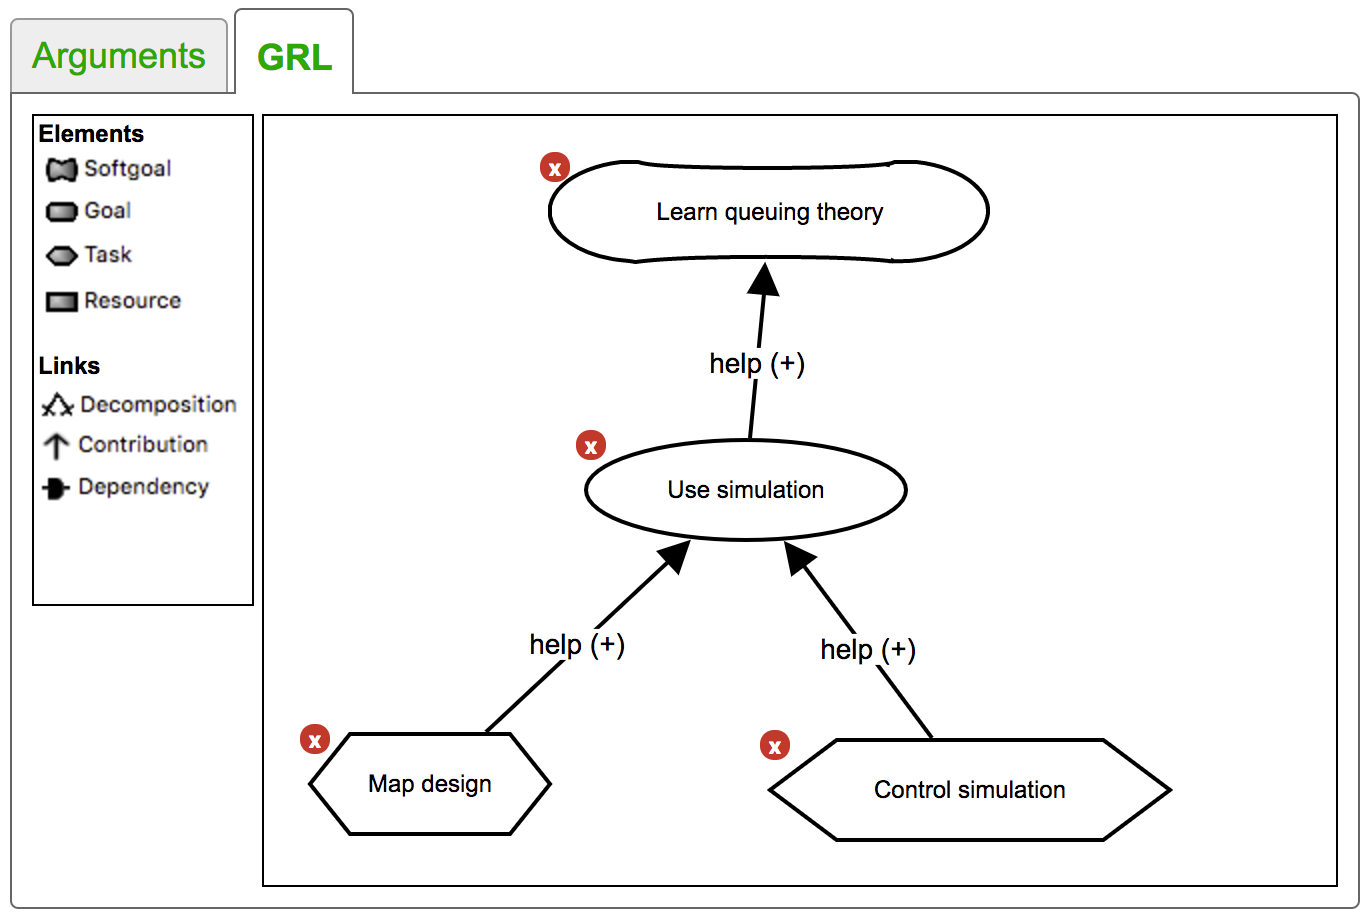
\includegraphics[scale=0.5]{img/tool_screen}
\caption{Screenshot of the prototype tool}
\label{fig:goalmodeling:tool}
\end{figure*}

An important aspect of the tool is that users can switch freely between these two ways of modeling the problem. One can model the entire problem in GRL, or one can do everything using argumentation. However, we believe the most powerful way to do so is to switch back and forth. For instance, one can create a simple goal model in GRL, and then turn to the argumentation part, which the users can look at the various critical questions for the elements, which may trigger discussions. These discussions results in new arguments for and against the elements in the goal model. Once this process is completed, one may switch to the goal model again, and so on. We believe that in this way, there is a close and natural coupling between modeling the goals of an organization as well as rationalizing them with arguments.